\documentclass[conference]{IEEEtran}
\IEEEoverridecommandlockouts
\usepackage[T1]{fontenc}
\usepackage[utf8]{inputenc}
\usepackage{amsmath,amssymb,booktabs,array,graphicx,url}
\usepackage[hidelinks]{hyperref}
\usepackage{enumitem,placeins,stfloats,float}
\graphicspath{{figures/}}
\setcounter{topnumber}{4}
\setcounter{dbltopnumber}{4}
\renewcommand{\topfraction}{0.95}
\renewcommand{\dbltopfraction}{0.95}
\renewcommand{\textfraction}{0.05}
\hypersetup{pdftitle={Project 4 Team 4 - Climate Analysis and Prediction},pdfauthor={Miguel A. De-Jesus-Rosa and Elias D Medina Galan}}
\setlength{\textfloatsep}{9pt plus 2pt minus 2pt}
\setlength{\floatsep}{8pt plus 2pt minus 2pt}
\newcommand{\figone}[3]{\begin{figure}[!tbp]\centering\includegraphics[width=\columnwidth]{#1}\caption{#2}\label{#3}\end{figure}}
\newcommand{\figwide}[3]{\begin{figure*}[!tbp]\centering\includegraphics[width=.97\textwidth]{#1}\caption{#2}\label{#3}\end{figure*}}
\title{Machine Learning in Climate Analysis and Prediction:\\Long-Term Trends, City Forecasts, Climate Zones, and Daily Weather Events}
\author{\IEEEauthorblockN{Miguel A. De-Jesus-Rosa and Elias D Medina Galan}
\IEEEauthorblockA{Computer Engineering Department\\Universidad Ana G. M\'endez, Gurabo Campus\\Gurabo, Puerto Rico\\mde472@email.uagm.edu}}
\begin{document}
\maketitle
\begin{abstract}
This study evaluates machine-learning methods for long-term temperature trends, city temperature forecasting, climate-zone discovery, and next-day rain and heat classification. Berkeley Earth temperature records, NOAA Mauna Loa carbon dioxide measurements, Australian weather observations, and Meteostat station data support five analysis phases. Chronological holdouts and training-fold preprocessing separate model development from evaluation. The global land-and-ocean series exhibits descriptive warming of 0.0360~$^\circ$C per decade during 1850--1974 and 0.1642~$^\circ$C per decade during 1975--2015, with ordinary-regression 95\% intervals of [0.0296, 0.0424] and [0.1405, 0.1878], respectively. Across ten cities, cross-validation-selected one-month models average 0.855~$^\circ$C test mean absolute error. A separate twelve-month Ridge experiment improves mean per-city error skill by 21.3\% over seasonal naive. Twenty-city clustering selects three groups but agrees weakly with detailed K\"oppen classes, with adjusted Rand index 0.0596. The selected rain support-vector machine achieves F1 0.640 and ROC-AUC 0.869; the heat random forest achieves F1 0.493 and ROC-AUC 0.878. These results demonstrate useful retrospective structure while exposing limitations in long-range extrapolation, climate-zone recovery, and reliable event warnings.
\end{abstract}
\begin{IEEEkeywords}climate analysis, machine learning, temperature forecasting, chronological validation, PCA, k-means, weather classification\end{IEEEkeywords}

\section{Introduction}
Climate records combine long-term change, repeatable seasonal behavior, and short-term variability. A model that captures one component may perform poorly on another. An annual temperature trend describes change over decades, whereas a next-day rain classifier must distinguish events using current meteorological conditions. Treating these questions as equivalent prediction problems obscures differences in information availability, target definition, and uncertainty.

Public data make it possible to study these scales together. Their convenience nevertheless introduces practical challenges: the city temperature file exceeds 8.5 million rows; historical coverage changes over time; rainfall observations contain missing values and an imbalanced target; and station archives may combine multiple providers. Model comparisons therefore require explicit selection, reproducible preprocessing, and forecast origins that prevent information from the future entering training.

This project addresses four research questions. \textbf{RQ1:} How fast did global temperature increase per decade, and how did its descriptive rate differ before and after 1975? \textbf{RQ2:} How accurately can monthly temperature be predicted in ten cities, including a twelve-month lead? \textbf{RQ3:} Do clusters of temperature climatologies reproduce established climate zones? \textbf{RQ4:} How well can next-day rain and heat be classified, and how has locally defined hot-day frequency changed?

The contribution is an integrated benchmark spanning data exploration, trend analysis, monthly forecasting, climate clustering, and daily event classification. Ten regression families are assessed for the one-month task; a separate twelve-month experiment evaluates Ridge and seasonal naive. Eight classification families are assessed for each event task. Descriptive trends and unsupervised diagnostics accompany the held-out scores but are not treated as equivalent predictive metrics.

\section{Related Work}
Reichstein \emph{et al.} connect learning from Earth-system data to process understanding, including temporal and spatial context \cite{reichstein}. This motivates seasonal features, historical lags, and the distinction between prediction and physical explanation. Our small tabular models differ from deep spatiotemporal architectures, making the comparison accessible within a course project without removing the need for physically meaningful interpretation.

Rolnick \emph{et al.} survey machine-learning applications to climate-change mitigation and adaptation \cite{rolnick}. Their work places predictions within broader decisions rather than making accuracy an end in itself. Here, heat and rainfall provide examples of why missed events and false alerts matter. The study measures prediction errors, but does not estimate avoided health impacts or energy savings from an operational system.

Ham, Kim, and Luo demonstrate deep-learning-based prediction of the El Ni\~no--Southern Oscillation at extended lead times \cite{ham}. That ocean--atmosphere target differs from city-level monthly air temperature. Their findings motivate investigating lead time, but cannot be transferred as expected accuracy for this dataset. We instead test a twelve-month Ridge hindcast restricted to information available at its forecast origin.

Rasp, Pritchard, and Gentine train a neural network to represent subgrid atmospheric processes within a climate model \cite{rasp}. This differs from direct statistical forecasting: a learned component substitutes for physical-process calculations. Our MLP uses historical tabular features and does not simulate atmospheric dynamics; retrospective accuracy cannot establish reliability under future forcing scenarios.

Beck \emph{et al.} provide K\"oppen--Geiger reference maps, with their 2023 product including historical 1961--1990 classes \cite{beck2018,beck2023}. Those classes incorporate precipitation as well as temperature. Disagreement with temperature-based clusters is therefore informative rather than automatically an implementation failure. We sample the historical raster at documented city centers.

Bergmeir, Hyndman, and Koo show that time-series cross-validation validity depends on assumptions such as residual dependence \cite{bergmeir}. We retain expanding temporal folds because nonstationarity and a prospective forecast setting are central here. Pedregosa \emph{et al.} describe the common scikit-learn framework used for consistent implementations \cite{pedregosa}. Relative to these works, this project emphasizes broad comparison, simple baselines, source auditing, and limitations rather than proposing a new algorithm.

\section{Data and Study Design}
\subsection{Sources and Coverage}
Table~\ref{tab:data} summarizes the source snapshot associated with the saved analysis. Temperatures use degrees Celsius and CO$_2$ uses parts per million. Berkeley Earth and Australian weather files came from versioned Kaggle distributions \cite{berkeley,kaggleberkeley,australia}; NOAA supplies CO$_2$ \cite{noaa}; Meteostat supplies the daily station product \cite{meteostat}. The analysis snapshot is dated October 30, 2026. Later updates must be treated as different source snapshots.
\begin{table}[t]
\caption{Source records before task-specific filtering. Dates refer to the saved snapshot.}\label{tab:data}\centering\footnotesize
\begin{tabular}{p{.28\columnwidth}r p{.43\columnwidth}}
\toprule Source & Rows & Coverage and spatial extent \\\midrule
Berkeley global & 3,192 & Jan. 1750--Dec. 2015; global aggregate \\
Berkeley cities & 8,599,212 & Nov. 1743--Sept. 2013; 3,510 geographic keys \\
NOAA CO$_2$ & 823 & Mar. 1958--Sept. 2026; Mauna Loa \\
Australian rain & 145,460 & Nov. 2007--June 2017; 49 locations \\
Meteostat 78526 & 9,445 & Jan. 2000--Dec. 2025; San Juan \\\bottomrule
\end{tabular}\end{table}
The global analysis uses \texttt{LandAndOceanAverageTemperature}, matching the integrated notebook. It is a blended global series rather than an unweighted city average or a land-only index. Trend estimation begins in 1850 and ends in 2015, the last complete year in this file; ``latest'' does not mean 2026. Earlier records remain useful for coverage auditing but are excluded from these trend fits.

The full city audit defines a geographic key using city, country, latitude, and longitude. Its 3,510 keys are not the number of distinct city--country pairs. Forecasting selects 24,851 rows for New York, London, Paris, Cairo, Bombay, Tokyo, Sydney, Cape Town, S\~ao Paulo, and La Plata. Bombay is the dataset identifier for Mumbai; La Plata replaces the suggested Buenos Aires because the latter was absent from the selected source. The selection spans both hemispheres and six inhabited continents.

Most cities provide 152 valid test months from January 2001 through August 2013; New York provides 153 through September 2013. The nominal 2001--2013 interval contains 156 months, so full-year 2013 coverage must not be claimed. Valid histories begin in 1743 for London, Paris, and New York, and between 1796 and 1857 elsewhere. Lag construction further reduces usable samples.

Station 78526 is San Juan International (ICAO TJSJ), at 18.4333$^\circ$N, 66.0000$^\circ$W and 3~m elevation \cite{meteostat}. It is a coastal regional reference, not a Gurabo-campus instrument. The daily provider is an aggregated product; the experiment does not establish that every value is directly observed or that the series is homogenized for trend analysis.

\subsection{Missing Data and Quality Control}
The audit records 7,224 missing cells in the global table, 728,260 in the city table, 585 in the loaded NOAA table, 343,248 in rain, and 38,551 in station data. These include different fields and table sizes and are not comparable percentages or counts of missing target labels. Source columns retained for auditing can be much less complete than fields used in a particular model.

City data are read in chunks of 250,000 rows, filtered, sorted, deduplicated by monthly date within city, and placed on a monthly calendar. Forecast rows with unavailable targets or required lag features are removed. No artificial observations or long-gap interpolations are introduced. Climatological means require at least twenty values for each calendar month during 1961--1990; all twenty selected profiles meet this rule.

NOAA dates are normalized from year and month, and nonpositive concentration codes become missing values. Rain rows require valid \texttt{RainTomorrow} labels. Numerical imputation uses the training-fold median; categorical imputation uses its most frequent category followed by one-hot encoding, ignoring unseen categories. Scaling is also fitted within each pipeline. Heat features use calendar shifts after reindexing to a daily calendar, so missing dates cannot masquerade as one-day lags.

\subsection{Partitions and Sampling}
One-month models train through December 2000 and test on available months in 2001--2013. Three expanding \texttt{TimeSeriesSplit} folds operate inside training. Prior observed months are available for successive one-month forecasts; the entire test period is not recursively forecast from a single initial date.

For the twelve-month task, the newest observed temperature feature is twelve months before its target. Training labels end in January 2000, consistent with information available at the first January 2001 target's origin. Cross-validation leaves an eleven-month gap. Target-month calendar variables are known in advance. This is a set of rolling-origin twelve-month hindcasts, not one forecast issued for the whole test interval.

Rain training ends in 2015 and testing begins in 2016. Among 142,193 valid labels, 116,219 belong to training and 25,974 to testing. Every classifier uses the same 24,000-row training subset, selected at uniformly spaced positions after date-and-location sorting to keep SVM computation practical. The complete test set is retained. Calendar-based CV groups observations from the same date and leaves a one-date gap; rain uses three folds.

Heat training ends in 2020; testing covers 2021--2025, the last five calendar years. Four expanding calendar-based folds operate within training. The heat test set contains 1,826 labels, including 236 positive cases. Test scores do not determine either event task's reporting model.

\figwide{eda_climate.pdf}{Four exploratory views: (a) annual global temperature and ten-year mean, (b) anomalies relative to 1951--1980, (c) NOAA CO$_2$, and (d) seasonal cycles in three cities. CO$_2$ after 2015 is displayed for context but excluded from the aligned temperature experiment.}{fig:eda}
\figwide{eda_rain.pdf}{Two additional exploratory views: RainTomorrow prevalence by location and the ten most incomplete rain fields. Prevalence excludes missing labels; missingness uses the original table.}{fig:rain_eda}

\section{Methods}
\subsection{Annual Anomalies and Trend Models}
Twelve monthly global values are averaged for each year; incomplete years are excluded. The 1951--1980 reference contains thirty complete annual means and has average temperature 15.300~$^\circ$C. Anomalies are
\begin{equation}A_y=T_y-\frac{1}{30}\sum_{k=1951}^{1980}T_k.\end{equation}
The ten-year moving mean requires ten annual values. Linear regression estimates $A_y=\beta_0+\beta_1 y+\epsilon_y$, with warming rate $10\hat\beta_1$. Descriptive fits cover 1850--1974, 1975--2015, and the combined period. Stored confidence intervals use the slope standard error and Student-$t$ critical value. They assume ordinary regression errors and do not adjust serial correlation.

Held-out trend experiments compare linear, quadratic, and cubic year functions. Training ends in 2000; testing covers 2001--2015. Four expanding training folds evaluate MAE. Ridge and Lasso compare year alone with year plus annual CO$_2$ over the common 1958--2015 interval. Their regularization search is $\alpha\in\{0.001,0.01,0.1,1,10,100\}$. Observed test-year CO$_2$ makes these conditional estimates rather than advance forecasts of unknown concentrations.

\subsection{Monthly Forecasting}
For target month $t$, one-month features are $T_{t-1}$, $T_{t-2}$, $T_{t-3}$, $T_{t-12}$, the preceding twelve-month mean, year, and
\begin{equation}\sin(2\pi m_t/12),\qquad\cos(2\pi m_t/12).\end{equation}
The seasonal-naive baseline is $\hat T_t=T_{t-12}$. Twelve-month Ridge uses lags 12, 13, 14, and 24, a twelve-month mean ending at $t-12$, and calendar features. Its baseline is again $T_{t-12}$, now the latest same-month value at its origin.

Linear regression supplies an unregularized reference; Ridge and Lasso shrink coefficients using $L_2$ and $L_1$ penalties. Polynomial regression expands standardized inputs to degree two and fits Ridge. k-NN predicts from nearby feature vectors. Decision trees learn thresholds; forests average multiple trees; gradient boosting adds trees sequentially. SVR models nonlinear relationships with an RBF kernel. The MLP uses a 32-unit hidden layer. These contrasting families test whether flexibility improves upon seasonal and linear structure.

Table~\ref{tab:search} gives the actual grids. Every forecast estimator uses a scaling pipeline. Search minimizes training CV MAE, and the reporting family is chosen separately for each city using that criterion. Linear regression and Naive Bayes receive CV with one specification because their implementation has no nontrivial tuning grid.
\begin{table*}[!tbp]
\caption{Executed search spaces; unlisted parameters use the executed library defaults. Stochastic estimators use seed 42 where supported.}\label{tab:search}\centering\footnotesize
\begin{tabular}{p{.16\textwidth}p{.39\textwidth}p{.37\textwidth}}
\toprule Family & Monthly regression & Rain and heat classification \\\midrule
Linear / Logistic & Ordinary least squares; one specification & Logistic $C\in\{0.1,1\}$; balanced classes \\
Ridge / Lasso & Ridge $\alpha\in\{0.1,1,10\}$; Lasso $\alpha\in\{0.001,0.01,0.1\}$ & Not applicable \\
Polynomial & Degree 2; Ridge $\alpha\in\{1,10\}$ & Not applicable \\
k-NN & Neighbors $\{3,7\}$ & Neighbors $\{9,25\}$ \\
Naive Bayes & Not applicable & Gaussian; one specification \\
Decision tree & Maximum depth $\{4,8\}$ & Maximum depth $\{5,10\}$; balanced classes \\
Random forest & 80 trees; depth $\{5,\mathrm{None}\}$ & 100 trees; depth $\{8,\mathrm{None}\}$; balanced classes \\
Gradient boosting & Estimators $\{80,120\}$ & Estimators $\{75,125\}$ \\
SVR / SVM & RBF; $C\in\{1,10\}$ & RBF; $C\in\{0.1,1\}$; balanced classes \\
MLP & Hidden layer (32); $\alpha\in\{0.001,0.1\}$; max. 2,500 iterations & Hidden layer (32); $\alpha\in\{0.001,0.1\}$; max. 1,500 iterations \\\bottomrule
\end{tabular}\end{table*}

\subsection{PCA and Climate Clustering}
Twenty cities are represented by twelve monthly 1961--1990 temperatures, their annual range, and latitude. Features are standardized before PCA and k-means. PCA supplies a two-dimensional view and interpretable loadings. K-means is fitted on all fourteen standardized features, not only the displayed components.

The search tests $k=2,\ldots,10$ with twenty initializations and seed 42. Inertia and silhouette guide selection. A Natural Earth basemap supports geographic visualization \cite{naturalearth}. Independent K\"oppen labels are sampled from Beck \emph{et al.}'s 1961--1990 raster at 0.1-degree resolution, from Figshare article 21789074 version 2 \cite{beck2023}. GeoNames supplies city-center points \cite{geonames}. Berkeley cell coordinates can differ from those city centers; this mismatch limits reference comparability. A contingency comparison and adjusted Rand index (ARI) avoid assuming numerical cluster IDs correspond directly to climate names.

\subsection{RainTomorrow and Hot-Day Classification}
Australian models predict tomorrow's rain using meteorological information recorded on the predictor date. Date, target labels, and possible future-rain proxy fields are excluded. Prediction is issued after the day's observations, permitting afternoon measurements. Logistic regression, k-NN, Gaussian Naive Bayes, SVM, decision tree, random forest, gradient boosting, and MLP share the same data and temporal folds.

Supported classifiers use balanced class weights; other families retain their standard objectives. Test data are not resampled, and thresholds are not optimized using test scores. CV maximizes F1. SVM ROC analysis uses its decision function rather than calibrated probabilities.

For heat, $q_{0.90}$ denotes the full-record 90th percentile of maximum temperature and $H_d=\mathbb{1}(T_{\max,d}>q_{0.90})$. The threshold is 32.2~$^\circ$C. Predicting day $d$ uses maximum-temperature lags 1, 2, 3, and 7, a seven-day mean ending on $d-1$, previous-day minimum temperature and precipitation, and cyclical month features. Target-day observed temperature is excluded.

The full-record label follows the assignment but is retrospective. The training-only percentile also equals 32.2~$^\circ$C in this snapshot, so labels coincide. That coincidence does not make full-record threshold estimation generally appropriate for deployment. Annual counts and rates are evaluated separately, retaining years with at least 90\% valid maximum-temperature coverage. Twenty-five years meet the rule.

\subsection{Metrics and Timing}
Forecast evaluation uses
\begin{equation}\mathrm{MAE}=\frac1n\sum_i|y_i-\hat y_i|,\quad\mathrm{RMSE}=\sqrt{\frac1n\sum_i(y_i-\hat y_i)^2},\end{equation}
and $R^2=1-\sum_i(y_i-\hat y_i)^2/\sum_i(y_i-\bar y)^2$. Skill is $1-E_{\rm model}/E_{\rm naive}$ on matching city months, averaged without population weighting. Mean city RMSE is distinguished from pooled RMSE.

Classification uses positive-class precision, recall, F1, ROC-AUC, and confusion matrices; rain accuracy is also reported by location. Reporting models use training CV F1. Search timings include CV, tuning, and refitting. Prediction time measures a batch \texttt{predict} call; classifier ROC-score computation is outside that interval. These are elapsed CPU timings with two search workers, not normalized deployment latency.

\section{Experimental Workflow: Implementation Steps}
The saved integrated run followed these steps:
\begin{enumerate}[leftmargin=*,itemsep=2pt]
\item Acquire or reuse versioned source files and record hashes of the exact snapshots.
\item Audit coverage, missingness, city identifiers, station metadata, and event labels; filter city data in chunks.
\item Construct annual anomalies, calendar features, temporal lags, climatologies, and targets; produce exploratory figures.
\item Establish chronological holdouts and folds; fit predictive preprocessing within training pipelines.
\item Evaluate trend models, ten regressors per city, the separate twelve-month Ridge experiment, and eight classifiers per event task.
\item Export PCA, k-means diagnostics, geographical maps, and twenty-city reference comparisons.
\item Interpret validation-selected models using residuals, confusion matrices, and permutation importance; save comparison tables and package versions.
\end{enumerate}
The master comparison contains 110 one-month rows, 20 twelve-month rows, sixteen classification rows, seven global predictive specifications, and two unsupervised diagnostic rows: 155 total. Their scientific roles differ, so a single score must not rank all tasks together. The notebook's nine sections and this paper's written-report structure are separate deliverable requirements.

\section{Results}
\subsection{Exploratory Patterns}
Figure~\ref{fig:eda}(a) shows interannual global variability around a rising long-term mean; its ten-year curve makes the late-record increase clearer. Figure~\ref{fig:eda}(b) expresses the same temperature record against a fixed baseline, avoiding interpretation based on an arbitrary absolute offset.

The CO$_2$ series in Fig.~\ref{fig:eda}(c) rises while retaining a seasonal cycle. Its longer coverage does not extend the temperature experiment past 2015. In Fig.~\ref{fig:eda}(d), Sydney's seasonal phase contrasts with London and Cairo. This supports cyclical month features and city-specific evaluation instead of an uninterpreted pooled seasonal profile.

Figure~\ref{fig:rain_eda}(a) shows substantial geographic variation in rain-label prevalence, making national accuracy insufficient for local assessment. Figure~\ref{fig:rain_eda}(b) shows especially incomplete cloud, evaporation, and sunshine fields. Imputation permits comparison but cannot remove bias from changing missingness. These six panels provide distinct exploration of trend, anomaly, CO$_2$, seasonality, class balance, and data quality.

\subsection{Warming and \texorpdfstring{CO$_2$}{CO2}}
Table~\ref{tab:slopes} reports descriptive rates. The 1975--2015 slope is approximately 4.56 times the earlier slope, differing by 0.1282~$^\circ$C per decade. This is a period comparison, not a formal breakpoint test. Ordinary intervals quantify uncertainty under their regression assumptions; serial dependence could alter coverage.
\begin{table}[t]\caption{Descriptive global land-and-ocean slopes; intervals assume ordinary regression errors.}\label{tab:slopes}\centering\footnotesize
\begin{tabular}{lcc}\toprule Period & $^\circ$C/decade & 95\% interval \\\midrule
1850--2015 & 0.0535 & [0.0486, 0.0584] \\
1850--1974 & 0.0360 & [0.0296, 0.0424] \\
1975--2015 & 0.1642 & [0.1405, 0.1878] \\\bottomrule\end{tabular}\end{table}
\begin{table*}[!tbp]\caption{Global test results, 2001--2015. CV is training MAE mean $\pm$ SD. Polynomial/linear training begins in 1850; Ridge/Lasso use 1958--2000. CO$_2$ models condition on observed test-year concentrations.}\label{tab:globalmodels}\centering\scriptsize
\begin{tabular}{llcrrrr}\toprule Model & Best parameters & CV MAE & MAE & RMSE & $R^2$ & Search (s) \\\midrule

Linear trend & {} & 0.182 $\pm$ 0.042 & 0.321 & 0.328 & -16.662 & 0.026 \\
Polynomial trend degree 2 & {} & 0.325 $\pm$ 0.227 & 0.147 & 0.161 & -3.231 & 0.032 \\
Polynomial trend degree 3 & {} & 0.479 $\pm$ 0.222 & 0.171 & 0.184 & -4.516 & 0.023 \\
Ridge & {'alpha': 1} & 0.130 $\pm$ 0.049 & 0.161 & 0.174 & -3.955 & 0.100 \\
Lasso & {'alpha': 0.01} & 0.131 $\pm$ 0.039 & 0.178 & 0.190 & -4.911 & 0.121 \\
Ridge + CO$_2$ & {'alpha': 0.1} & 0.093 $\pm$ 0.027 & 0.101 & 0.119 & -1.313 & 0.114 \\
Lasso + CO$_2$ & {'alpha': 0.001} & 0.102 $\pm$ 0.038 & 0.092 & 0.109 & -0.956 & 0.102 \\

\bottomrule\end{tabular}\end{table*}
All seven global predictive specifications have negative test $R^2$ (Table~\ref{tab:globalmodels}). Smooth descriptive fits therefore do not establish reliable extrapolation relative to the test-period mean. Quadratic regression reduces MAE relative to the full-history linear model but still has $R^2=-3.231$.

On the common-period comparisons, CO$_2$ reduces Ridge MAE from 0.161 to 0.101~$^\circ$C and Lasso MAE from 0.178 to 0.092~$^\circ$C. Lasso plus CO$_2$ has the smallest conditional test MAE, but $R^2$ remains negative ($-0.956$). The result supports an association in this snapshot, not causal attribution or unconditional forecasting success.

\subsection{One-Month City Forecasts}
Table~\ref{tab:regression} reports every required family. Polynomial regression has the smallest mean city test MAE, 0.829~$^\circ$C, versus 1.179~$^\circ$C for seasonal naive. This is a retrospective test summary, not the selection rule. Linear, Ridge, and Lasso remain competitive, whereas the decision tree is close to baseline on average.
\begin{table*}[!tbp]\caption{One-month comparison: unweighted means across ten cities. CV columns average each city's selected configuration's fold mean and fold SD; they are not pooled intervals. Times are means per city. Exact parameters and all 110 rows accompany the source package.}\label{tab:regression}\centering\footnotesize
\begin{tabular}{lrrrrrrr}\toprule Model & CV MAE & CV SD & Test MAE & Test RMSE & Test $R^2$ & Search (s) & Predict (s) \\\midrule

Seasonal naive & -- & -- & 1.179 & 1.491 & 0.857 & 0.00 & 0.0000 \\
Linear & 0.890 & 0.029 & 0.871 & 1.112 & 0.915 & 0.03 & 0.0007 \\
Ridge & 0.890 & 0.029 & 0.871 & 1.112 & 0.915 & 0.05 & 0.0007 \\
Lasso & 0.889 & 0.028 & 0.873 & 1.114 & 0.914 & 0.05 & 0.0006 \\
Polynomial & 0.940 & 0.109 & 0.829 & 1.052 & 0.926 & 0.05 & 0.0017 \\
kNN & 0.942 & 0.050 & 0.924 & 1.167 & 0.911 & 0.05 & 0.0132 \\
Decision tree & 1.051 & 0.042 & 1.167 & 1.458 & 0.858 & 0.05 & 0.0008 \\
Random forest & 0.922 & 0.031 & 0.964 & 1.202 & 0.909 & 1.07 & 0.0238 \\
Gradient boosting & 0.962 & 0.049 & 0.935 & 1.178 & 0.913 & 1.02 & 0.0013 \\
SVR & 1.407 & 0.427 & 0.920 & 1.158 & 0.911 & 0.43 & 0.0092 \\
MLP & 1.457 & 0.377 & 0.924 & 1.176 & 0.891 & 4.33 & 0.0012 \\

\bottomrule\end{tabular}\end{table*}
Validation-selected reporting families differ by city (Table~\ref{tab:cities}) and average 0.855~$^\circ$C test MAE. Bombay has the smallest selected-model MAE, 0.442~$^\circ$C; New York and Paris have larger errors of 1.305 and 1.277~$^\circ$C. These are conditional results, not an intrinsic city-predictability ranking independent of variability and source quality.
\begin{table*}[!tbp]\caption{City reporting models selected using training CV, with exact best parameters. CV is MAE mean $\pm$ SD across three training folds.}\label{tab:cities}\centering\scriptsize
\begin{tabular}{lllcrrr}\toprule City & Family & Best parameters & CV MAE & Test MAE & Test RMSE & Test $R^2$ \\\midrule

Bombay & Polynomial & {'alpha': 10, 'degree': 2} & 0.459 $\pm$ 0.005 & 0.442 & 0.543 & 0.865 \\
Cairo & Linear & {} & 0.791 $\pm$ 0.007 & 0.794 & 1.002 & 0.969 \\
Cape Town & Lasso & {'alpha': 0.001} & 0.653 $\pm$ 0.037 & 0.568 & 0.707 & 0.945 \\
La Plata & Lasso & {'alpha': 0.01} & 0.951 $\pm$ 0.028 & 0.939 & 1.198 & 0.938 \\
London & Ridge & {'alpha': 10} & 1.147 $\pm$ 0.048 & 1.013 & 1.324 & 0.931 \\
New York & Lasso & {'alpha': 0.01} & 1.282 $\pm$ 0.027 & 1.305 & 1.658 & 0.967 \\
Paris & Ridge & {'alpha': 1} & 1.287 $\pm$ 0.045 & 1.277 & 1.662 & 0.919 \\
Sydney & Lasso & {'alpha': 0.01} & 0.607 $\pm$ 0.025 & 0.580 & 0.750 & 0.869 \\
S\~ao Paulo & Polynomial & {'alpha': 10, 'degree': 2} & 0.718 $\pm$ 0.033 & 0.779 & 0.965 & 0.829 \\
Tokyo & Polynomial & {'alpha': 10, 'degree': 2} & 0.882 $\pm$ 0.010 & 0.850 & 1.087 & 0.982 \\

\bottomrule\end{tabular}\end{table*}
\figwide{phase3_forecast_Bombay.png}{Bombay forecast detail: actual observations, seasonal naive, and CV-selected Polynomial. The early-test view illustrates seasonal tracking; metrics use all available held-out months.}{fig:bombay}
\figone{phase3_forecast_Cairo.png}{Cairo forecast detail with the CV-selected Linear model.}{fig:cairo}
\figone{phase3_forecast_Cape_Town.png}{Cape Town forecast detail with the CV-selected Lasso model.}{fig:cape}
Figures~\ref{fig:bombay}--\ref{fig:cape} illustrate strong seasonal tracking in three cities. Deviations remain: reproducing the typical seasonal peak is easier than predicting every unusually warm or cool month. All ten cities remain represented in the numerical comparison.

\subsection{Twelve-Month Lead}
Twelve-month Ridge improves over seasonal naive in all ten cities. Its mean city MAE is 0.919~$^\circ$C, compared with 1.179~$^\circ$C for baseline. Mean city RMSE is 1.165~$^\circ$C and mean city $R^2$ is 0.907. Averaging the relative MAE skill within each city yields 21.3\%; this differs from taking the ratio of aggregate MAEs.
\figwide{horizon.pdf}{Ridge error at one- and twelve-month leads, and twelve-month skill over seasonal naive. Only Ridge and the baseline were tested at twelve months.}{fig:horizon}
Figure~\ref{fig:horizon} shows variation across cities: twelve-month skill is 26.9\% for New York, 27.4\% for Cape Town, and 11.3\% for Bombay. Comparing Ridge at the two leads is informative, but feature sets and purged endpoints differ. The experiment cannot determine which of ten families degrades fastest, because nine families were not run at twelve months.

\subsection{Climate Structure and Reference Agreement}
The first two PCs explain 62.9\% and 33.7\% of standardized-profile variance (96.6\% combined). PC1 loads positively on monthly temperatures and negatively on annual range; PC2 contrasts seasonal patterns. These descriptions interpret this sample's loadings rather than define universal climate coordinates.
\figone{phase4_pca.png}{PCA of twenty standardized climatologies, annual range, and latitude. Two components explain 96.6\% of sample variance.}{fig:pca}
\figone{phase4_cluster_diagnostics.png}{K-means diagnostics for $k=2$--10. Silhouette peaks at 0.608 for three groups.}{fig:clusterdiag}
The PCA in Fig.~\ref{fig:pca} exposes broad temperature/seasonality structure. Figure~\ref{fig:clusterdiag} favors $k=3$: inertia drops from 141.24 to 49.73 between two and three clusters, and silhouette peaks at 0.6076. Further clusters reduce inertia but have lower silhouettes.
\figwide{phase4_geo_clusters.png}{World distribution of three temperature-based groups, using Berkeley coordinates. Reference labels are independently sampled at GeoNames city centers. Basemap: Natural Earth, public domain.}{fig:world}
\begin{table}[t]\caption{Twenty-city comparison. Coordinates are Berkeley temperature-cell coordinates; K\"oppen labels use independently sampled city centers. Cluster IDs are arbitrary.}\label{tab:koppen}\centering\scriptsize
\begin{tabular}{lccrr}\toprule City & Cluster & K\"oppen & Latitude & Longitude \\\midrule

Bangkok & 2 & Aw & 13.66 & 99.91 \\
Berlin & 1 & Dfb & 52.24 & 13.14 \\
Bombay & 2 & Am & 18.48 & 72.68 \\
Cairo & 2 & BWh & 29.74 & 31.38 \\
Cape Town & 0 & Csb & -32.95 & 18.19 \\
Chicago & 1 & Dfa & 42.59 & -87.27 \\
La Plata & 0 & Cfa & -34.56 & -58.38 \\
Lima & 0 & BWh & -12.05 & -77.26 \\
London & 1 & Cfb & 52.24 & -0.00 \\
Los Angeles & 1 & Csa & 34.56 & -118.70 \\
Melbourne & 0 & Cfb & -37.78 & 144.41 \\
Moscow & 1 & Dfb & 55.45 & 36.85 \\
Nairobi & 0 & Cfb & -0.80 & 36.16 \\
New York & 1 & Dfa & 40.99 & -74.56 \\
Paris & 1 & Cfb & 49.03 & 2.45 \\
Peking & 1 & Dwa & 39.38 & 116.53 \\
Singapore & 2 & Af & 0.80 & 103.66 \\
Sydney & 0 & Cfa & -34.56 & 151.78 \\
S\~ao Paulo & 0 & Cfa & -23.31 & -46.31 \\
Tokyo & 1 & Cfa & 36.17 & 139.23 \\

\bottomrule\end{tabular}\end{table}
The map in Fig.~\ref{fig:world} has broad hemispheric structure: cluster 0 contains Southern Hemisphere cities, cluster 1 includes many Northern Hemisphere seasonal profiles, and cluster 2 includes warm tropical/subtropical profiles. Yet Cairo and Singapore share cluster 2 despite BWh and Af reference classes. Lima and Cape Town share cluster 0 despite BWh and Csb (Table~\ref{tab:koppen}). ARI is only 0.0596. A good silhouette establishes separation in the selected space, not recovery of detailed K\"oppen zones. Omitted precipitation and calendar phase plausibly explain part of this mismatch.

\begin{figure}[H]\centering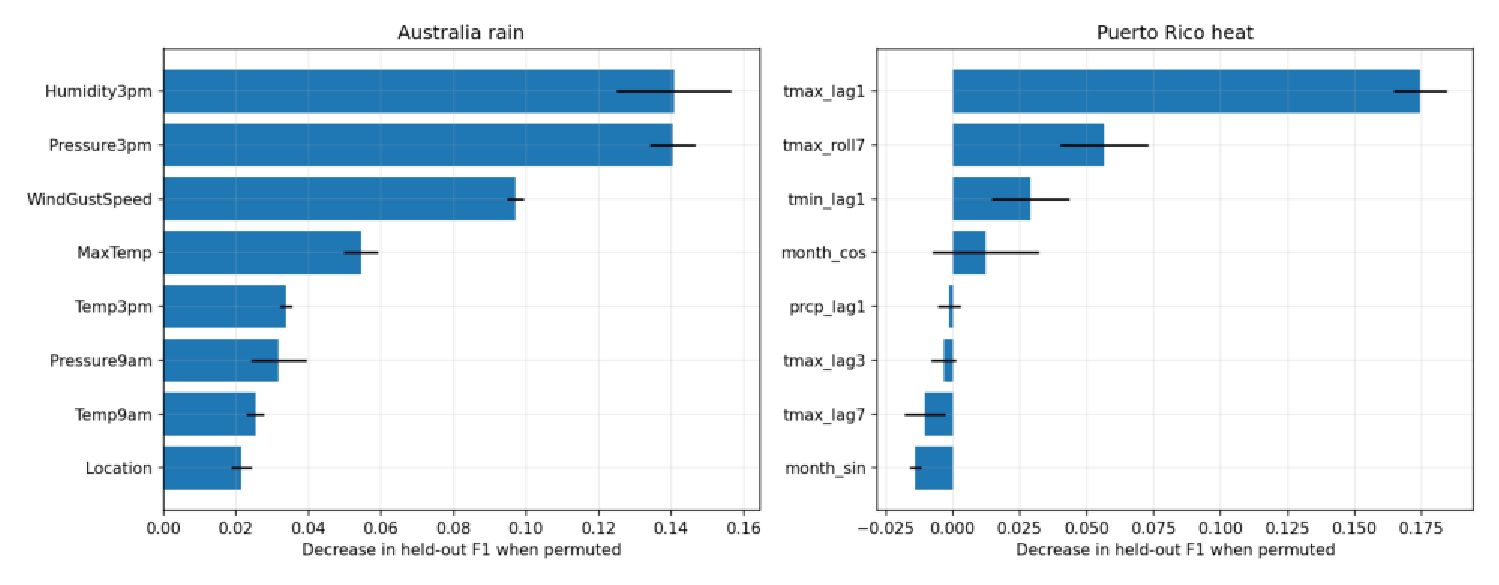
\includegraphics[width=\columnwidth]{importance_compact.pdf}
\caption{Permutation importance for CV-selected classifiers on fixed 1,000-row test samples, three repeats. Bars show F1 reduction after permutation and repeat variability.}\label{fig:importance}\end{figure}
\subsection{Next-Day Rain and Heat}
Tables~\ref{tab:rain} and \ref{tab:heat} contain all event families. Rain SVM is selected because its training CV F1 is highest, 0.645. Test F1 is 0.640, ROC-AUC is 0.869, recall is 76.7\%, and precision is 55.0\%. MLP has slightly higher test AUC, 0.874, but is not substituted after seeing that result.
\begin{table*}[!tbp]\caption{Rain classification on 25,974 test rows, using the shared 24,000-row training sample. CV is F1 mean $\pm$ SD. Times include search/refit and batch class prediction.}\label{tab:rain}\centering\scriptsize
\begin{tabular}{llcrrrrrr}\toprule Model & Best parameters & CV F1 & Precision & Recall & F1 & ROC-AUC & Search (s) & Predict (s) \\\midrule

Logistic & {'C': 0.1} & 0.633 $\pm$ 0.013 & 0.527 & 0.744 & 0.617 & 0.856 & 2.87 & 0.156 \\
kNN & {'n\_neighbors': 9} & 0.519 $\pm$ 0.023 & 0.703 & 0.424 & 0.529 & 0.826 & 1.76 & 2.762 \\
Naive Bayes & {} & 0.486 $\pm$ 0.022 & 0.348 & 0.692 & 0.463 & 0.720 & 0.35 & 0.116 \\
SVM & {'C': 1} & 0.645 $\pm$ 0.010 & 0.550 & 0.767 & 0.640 & 0.869 & 66.39 & 20.535 \\
Decision tree & {'max\_depth': 5} & 0.573 $\pm$ 0.014 & 0.463 & 0.739 & 0.569 & 0.820 & 0.81 & 0.043 \\
Random forest & {'max\_depth': 8} & 0.622 $\pm$ 0.012 & 0.511 & 0.719 & 0.597 & 0.839 & 3.90 & 0.104 \\
Gradient boosting & {'n\_estimators': 125} & 0.585 $\pm$ 0.024 & 0.733 & 0.482 & 0.582 & 0.857 & 23.98 & 0.103 \\
MLP & {'alpha': 0.1} & 0.621 $\pm$ 0.023 & 0.724 & 0.552 & 0.627 & 0.874 & 14.31 & 0.063 \\

\bottomrule\end{tabular}\end{table*}
\begin{table*}[!tbp]\caption{San Juan heat classification, 1,826 test days in 2021--2025. Threshold: full-record 90th percentile (32.2~$^\circ$C). CV is training F1 mean $\pm$ SD.}\label{tab:heat}\centering\scriptsize
\begin{tabular}{llcrrrrrr}\toprule Model & Best parameters & CV F1 & Precision & Recall & F1 & ROC-AUC & Search (s) & Predict (s) \\\midrule

Logistic & {'C': 1} & 0.303 $\pm$ 0.029 & 0.282 & 0.886 & 0.428 & 0.876 & 0.27 & 0.033 \\
kNN & {'n\_neighbors': 9} & 0.146 $\pm$ 0.094 & 0.613 & 0.288 & 0.392 & 0.818 & 0.36 & 0.058 \\
Naive Bayes & {} & 0.293 $\pm$ 0.037 & 0.290 & 0.839 & 0.431 & 0.859 & 0.08 & 0.014 \\
SVM & {'C': 1} & 0.295 $\pm$ 0.032 & 0.301 & 0.928 & 0.454 & 0.869 & 3.21 & 0.241 \\
Decision tree & {'max\_depth': 5} & 0.299 $\pm$ 0.036 & 0.303 & 0.864 & 0.448 & 0.862 & 0.22 & 0.015 \\
Random forest & {'max\_depth': 8} & 0.326 $\pm$ 0.057 & 0.362 & 0.771 & 0.493 & 0.878 & 2.50 & 0.038 \\
Gradient boosting & {'n\_estimators': 125} & 0.279 $\pm$ 0.062 & 0.644 & 0.322 & 0.429 & 0.885 & 2.96 & 0.016 \\
MLP & {'alpha': 0.001} & 0.110 $\pm$ 0.090 & 0.685 & 0.212 & 0.324 & 0.876 & 2.18 & 0.015 \\

\bottomrule\end{tabular}\end{table*}
Heat random forest has the highest CV F1, 0.326, and test F1 0.493. Test AUC is 0.878, recall 77.1\%, and precision 36.2\%. Gradient boosting has higher test AUC but much lower positive recall at its default decision rule. Ranking quality and usefulness at a particular threshold therefore differ.
\figone{phase5_rain_roc.png}{Rain ROC curves for all eight families on the holdout; the diagonal indicates chance ranking.}{fig:rainroc}
\figone{phase5_heat_roc.png}{Heat ROC curves. Similar AUC can coexist with markedly different precision and recall.}{fig:heatroc}
Figures~\ref{fig:rainroc} and \ref{fig:heatroc} show discrimination beyond chance but do not establish calibration or safe alert thresholds. Naive Bayes is weaker for rain ranking. Heat curves are closer even where F1 differs substantially.
\figone{confusions.pdf}{CV-selected model confusion matrices. Rain SVM misses 1,386 events and produces 3,733 false alarms. Heat random forest misses 54 events and produces 321 false alarms.}{fig:confusions}
Rain accuracy is 80.3\%, with 5,946 positive labels among 25,974 cases (22.9\%). An always-no-rain rule already achieves 77.1\% accuracy while detecting no rain. Heat accuracy is 79.5\%, below the 87.1\% always-no-heat accuracy, but that trivial rule has zero recall. Figure~\ref{fig:confusions} exposes the practical tradeoff masked by accuracy.

Rain per-location accuracy ranges from 66.2\% at Cairns (494 cases) to 93.2\% at Uluru (533 cases). The full forty-nine-location table accompanies the source. National averages do not establish uniform local performance, and evaluation at observed locations does not prove transfer to unseen stations.

\subsection{Hot-Day Trend and Error Analysis}
For twenty-five high-coverage years, annual hot-day counts increase by a fitted 0.846 days/year, or 8.46 days/decade. The valid-day rate increases by 2.20 percentage points/decade. An additional ordinary-regression analysis of the saved annual table gives count-slope 95\% interval $[-1.88,18.79]$ days/decade ($p=0.104$) and rate-slope interval $[-0.65,5.06]$ percentage points/decade ($p=0.124$). Thus the positive fitted trend is not distinguishable from zero at the 5\% level under this simple model. These additional report calculations do not adjust serial correlation.
\figone{phase5_heat_trend.png}{Hot-day counts for years with at least 90\% valid daily maxima. The fitted upward line is descriptive; its ordinary slope interval includes zero.}{fig:heattrend}
Figure~\ref{fig:heattrend} shows large annual variation, including a late-record peak, rather than a steady yearly increase. Counts are sensitive to valid-day coverage; the rate partially addresses denominators but cannot correct provider changes or station history.
\figone{residual_compact.pdf}{Post-evaluation monthly-model diagnostics: seasonal MAE and actual-minus-predicted residuals. Diagnostics do not determine model selection.}{fig:residuals}

Selected-model mean residuals are positive in all ten cities, from 0.044~$^\circ$C in Cape Town to 0.475~$^\circ$C in Paris, indicating average underprediction. New York's maximum absolute error is 4.93~$^\circ$C. Figure~\ref{fig:residuals} shows that typical MAE does not bound individual errors and that performance varies seasonally.

In Fig.~\ref{fig:importance}, Humidity3pm, Pressure3pm, and WindGustSpeed dominate rain permutation importance. Previous-day maximum temperature, its trailing seven-day mean, and previous-day minimum temperature dominate heat importance. Correlated features can divide importance; slightly negative estimates can reflect sampling noise. These are predictive diagnostics rather than causal effects.

\FloatBarrier
\section{Discussion}
\subsection{Answers to the Research Questions}
\textbf{RQ1: Warming rates.} The observed global land-and-ocean series has larger descriptive warming in 1975--2015 than 1850--1974: 0.1642 versus 0.0360~$^\circ$C/decade. Ordinary intervals are available, but a formal slope-break test and autocorrelation-adjusted inference were not completed. The result is a descriptive period difference, not a new attribution analysis. Broader physical attribution is addressed by assessment literature \cite{ipcc2023}.

\textbf{RQ2: Forecasts.} CV-selected one-month models average 0.855~$^\circ$C MAE. Twelve-month Ridge averages 0.919~$^\circ$C MAE and 21.3\% mean city skill over seasonal naive. Flexible families are not universally superior, and the full ten-family comparison at twelve months remains future work.

\textbf{RQ3: Climate zones.} Three clusters separate the standardized sample reasonably well, but ARI 0.0596 shows weak agreement with detailed K\"oppen classes. Seasonality, latitude, and hemisphere produce broad groups without precipitation-based distinctions. The analysis discovers temperature patterns rather than replaces established climate classification.

\textbf{RQ4: Events and frequency.} Rain and heat reporting models detect many positives, with recalls 76.7\% and 77.1\%, but false alarms and missed events remain material. Hot-day counts have a positive fitted slope, yet the ordinary interval includes zero. This station-specific evidence does not establish a campus-wide or island-wide trend.

\subsection{Required Discussion Questions}
\textbf{Does CO$_2$--temperature association prove causation?} No. Conditional errors improve here, but year and CO$_2$ share temporal trends and correlated predictors can have unstable coefficients. Attribution also needs physical mechanisms, competing forcings, internal variability, and suitable causal or physical analysis. The limitations of this simple regression do not weaken the wider physical evidence summarized by the IPCC \cite{ipcc2023}.

\textbf{Why can forecasts worsen with lead time, and which degrade fastest?} Recent weather measurements are unavailable at longer leads, unpredictable innovations accumulate, and recursive models can propagate errors. Ridge's average error increases here, although individual cities vary. Only Ridge was tested at both leads, so the fastest-degrading family is not established. A fair comparison needs common origins and multi-horizon experiments for all families.

\textbf{How can instruments, station moves, and sparse early data bias trends?} Instrument changes and relocation can introduce discontinuities. Urbanization changes exposure; changing geographic coverage can shift an unweighted average even without common local change. Missing months can alter annual seasonal composition. Complete-year and high-coverage filters address some consequences but cannot replace homogenization, metadata checks, and robust uncertainty analysis.

\textbf{How could heat predictions support planning?} Independent local validation could support reviewing cooling resources, outreach staffing, or electricity demand. Action thresholds should reflect missed-event and false-alert costs. The selected model produces 321 false alerts for 182 true positive days; direct automated warnings require further evaluation. A station percentile is not a clinical heat-risk threshold. Humidity, exposure, vulnerability, and calibration would be needed for specific public-health interventions.

\subsection{Limitations}
Files end at different times; global analysis ends in 2015. Ten forecasting cities and twenty clustering cities cannot represent all climates. Berkeley grid coordinates and independently sampled city centers can differ. San Juan International is a regional airport record, and aggregated provider data do not guarantee observation-only provenance.

The rain sample discards available training observations to permit common-family comparison. Small grids and one seed do not establish optimal performance. CV standard deviations summarize folds rather than population confidence intervals. Source uncertainty is explored but not propagated through predictions. Warming intervals assume ordinary errors; no robust breakpoint test was performed. Full-record heat labeling is retrospective even though training-only and full-record thresholds coincide in this snapshot.

Default classifier decisions are retained without validation-only threshold tuning or probability calibration. Residual and importance analyses are post-evaluation interpretations; reusing them to tune models would require a new validation strategy. Statistical fit and positive silhouette cannot substitute for physical validation or operational reliability.

\section{Conclusion and Future Work}
The integrated study finds larger descriptive warming after 1975, useful seasonal temperature prediction, weak recovery of detailed K\"oppen zones, and daily event classifiers limited by decision errors. CV-selected one-month models average 0.855~$^\circ$C MAE; twelve-month Ridge supplies 21.3\% mean city skill over seasonal naive. Rain SVM and heat random forest achieve F1 0.640 and 0.493. Local annual hot-day counts have a positive fitted slope whose ordinary interval includes zero.

Future work should extend all regressors to common multi-horizon tests, add precipitation to clustering, assess geographic transfer, audit station history, and use temporally robust uncertainty estimates. Operational heat modeling requires a frozen past-only reference, calibrated risk, and independent local validation. Results should support transparent comparisons rather than causal claims from association or immediate deployment.

\section*{Reproducibility and Data Availability}
The source package contains this manuscript, figures, exact tables, a 155-row master comparison, source hashes, and tested versions. The evidence comes from the saved integrated notebook \texttt{ProjectX\_Team4.ipynb} and its October 30, 2026 outputs. This does not claim the older linked live notebook was fully rerun after its separate acquisition correction. The saved run executed 27 code cells in an in-process IPython executor using cached sources; fresh Google-hosted end-to-end acquisition was not verified for that run.

The environment used Python 3.12.14, NumPy 2.3.5, pandas 3.1.0, scikit-learn 1.8.0, SciPy 1.17.0, Matplotlib 3.10.8, seaborn 0.13.2, kagglehub 1.0.3, Meteostat 2.1.5, and rasterio 1.5.2. Search used two workers. Processor model and total memory were not recorded, so timings remain execution-specific. Source manifests identify exact cached bytes; large raw data are excluded from the report package.

The project repository is \url{https://github.com/Edariel22/Project4_Climate_Analysis}. A matching committed manuscript revision has not yet been established; this report does not assert these deliverables are uploaded there. Codex assisted with notebook revisions, report drafting, and formatting. Both students must verify the results and follow the course AI-assistance policy.

\begin{thebibliography}{00}
\bibitem{reichstein} M. Reichstein \emph{et al.}, ``Deep learning and process understanding for data-driven Earth system science,'' \emph{Nature}, vol. 566, pp. 195--204, 2019, doi: 10.1038/s41586-019-0912-1.
\bibitem{rolnick} D. Rolnick \emph{et al.}, ``Tackling climate change with machine learning,'' \emph{ACM Computing Surveys}, vol. 55, no. 2, Art. 42, 2022, doi: 10.1145/3485128.
\bibitem{ham} Y.-G. Ham, J.-H. Kim, and J.-J. Luo, ``Deep learning for multi-year ENSO forecasts,'' \emph{Nature}, vol. 573, pp. 568--572, 2019, doi: 10.1038/s41586-019-1559-7.
\bibitem{rasp} S. Rasp, M. S. Pritchard, and P. Gentine, ``Deep learning to represent subgrid processes in climate models,'' \emph{Proc. Natl. Acad. Sci. USA}, vol. 115, pp. 9684--9689, 2018, doi: 10.1073/pnas.1810286115.
\bibitem{beck2018} H. E. Beck \emph{et al.}, ``Present and future K\"oppen--Geiger climate classification maps at 1-km resolution,'' \emph{Scientific Data}, vol. 5, Art. 180214, 2018, doi: 10.1038/sdata.2018.214.
\bibitem{beck2023} H. E. Beck \emph{et al.}, ``High-resolution (1 km) K\"oppen--Geiger maps for 1901--2099 based on constrained CMIP6 projections,'' \emph{Scientific Data}, vol. 10, Art. 724, 2023, doi: 10.1038/s41597-023-02549-6. Historical data: Figshare 21789074, version 2.
\bibitem{bergmeir} C. Bergmeir, R. J. Hyndman, and B. Koo, ``A note on the validity of cross-validation for evaluating autoregressive time series prediction,'' \emph{Computational Statistics \& Data Analysis}, vol. 120, pp. 70--83, 2018, doi: 10.1016/j.csda.2017.11.003.
\bibitem{pedregosa} F. Pedregosa \emph{et al.}, ``Scikit-learn: Machine learning in Python,'' \emph{Journal of Machine Learning Research}, vol. 12, pp. 2825--2830, 2011.
\bibitem{berkeley} Berkeley Earth, ``Temperature data.'' [Online]. Available: \url{https://berkeleyearth.org/data/}. Accessed: Oct. 30, 2026.
\bibitem{kaggleberkeley} Berkeley Earth, ``Climate change: Earth surface temperature data,'' Kaggle, version 2. [Online]. Available: \url{https://www.kaggle.com/datasets/berkeleyearth/climate-change-earth-surface-temperature-data}. Accessed: Oct. 30, 2026.
\bibitem{australia} Kaggle user jsphyg, ``Rain in Australia,'' Kaggle, \texttt{jsphyg/weather-dataset-rattle-package}, version 2. [Online]. Available: \url{https://www.kaggle.com/datasets/jsphyg/weather-dataset-rattle-package}. Accessed: Oct. 30, 2026.
\bibitem{noaa} NOAA Global Monitoring Laboratory, ``Trends in atmospheric carbon dioxide: Mauna Loa monthly means.'' [Online]. Available: \url{https://gml.noaa.gov/ccgg/trends/}. Accessed: Oct. 30, 2026.
\bibitem{meteostat} Meteostat, ``San Juan / Int., station 78526.'' [Online]. Available: \url{https://meteostat.net/en/station/78526}. Accessed: Oct. 30, 2026.
\bibitem{naturalearth} Natural Earth, ``1:110m cultural vectors: Admin 0 countries,'' public-domain basemap. [Online]. Available: \url{https://www.naturalearthdata.com/}.
\bibitem{geonames} GeoNames, ``Geographical database: cities15000,'' CC BY 4.0. [Online]. Available: \url{https://download.geonames.org/export/dump/}.
\bibitem{ipcc2023} IPCC, \emph{Climate Change 2023: Synthesis Report}. Geneva, Switzerland: IPCC, 2023. [Online]. Available: \url{https://www.ipcc.ch/report/ar6/syr/}.
\end{thebibliography}

\section*{Author Contributions}
The author list follows the supplied template. Elias D Medina Galan's full name has been confirmed by the team; contact information has not been supplied. Specific tasks must be confirmed against actual work and commit history; file ownership does not establish authorship of individual analyses.
\begin{table}[h]\centering\footnotesize
\begin{tabular}{p{.30\columnwidth}p{.60\columnwidth}}
\toprule Author & Contribution record \\\midrule
Miguel A. De-Jesus-Rosa & Coding, analysis, writing, and commit evidence require author confirmation. \\
Elias D Medina Galan & Coding, analysis, writing, and commit evidence require author confirmation. \\\bottomrule
\end{tabular}\end{table}
\end{document}
